\documentclass[12pt,a4paper]{article}
\usepackage{etoc}
\usepackage[utf8]{vietnam}
\usepackage[top=2cm, bottom=2cm, left=2cm, right=2cm]{geometry}
\usepackage{amsmath,amsfonts,amssymb}
\usepackage{indentfirst,enumitem}
\usepackage{graphicx}
\usepackage{multicol}
\usepackage{setspace}
\usepackage{hyperref}
\usepackage{listings}
\usepackage{tabularx}
\usepackage{hyperref}
\usepackage{xcolor}
\usepackage{scrextend}
\usepackage{comment}
\usepackage{soul}
\usepackage{tikz,tkz-tab}
\usepackage{array}
%\changefontsizes{13pt}
\renewcommand*{\thesection}{\Roman{section}}
\renewcommand*{\thesubsection}{\arabic{subsection}}
\renewcommand*{\thesubsubsection}{\arabic{subsection}.\arabic{subsubsection}}

%New colors defined below
\definecolor{codegreen}{rgb}{0,0.6,0}
\definecolor{codegray}{rgb}{0.5,0.5,0.5}
\definecolor{codepurple}{rgb}{0.58,0,0.82}
\definecolor{backcolour}{rgb}{0.95,0.95,0.92}
\definecolor{Danube}{RGB}{91, 155, 213}
%Code listing style named "mystyle"
\lstdefinestyle{mystyle}{
  backgroundcolor=\color{backcolour},   commentstyle=\color{codegreen},
  keywordstyle=\color{blue},
  numberstyle=\tiny\color{codegray},
  stringstyle=\color{codepurple},
  basicstyle=\ttfamily\footnotesize,
  breakatwhitespace=false,         
  breaklines=true,                 
  captionpos=b,                    
  keepspaces=true,                 
  numbers=left,                    
  numbersep=5pt,                  
  showspaces=false,                
  showstringspaces=false,
  showtabs=false,                  
  tabsize=2
}

%"mystyle" code listing set
\lstset{style=mystyle}

\begin{document}
\begin{titlepage}
    %\SetWatermarkText{\includegraphics[width = 0.97\paperwidth,
    %height = 0.97\paperheight]{bia.png}}
    %\SetWatermarkAngle{0} 
    %\SetWatermarkText{\includegraphics[scale=1]{hust.png}}
    %\SetWatermarkAngle{0} 
    \begin{tikzpicture}[remember picture,overlay,inner sep=0,outer sep=0]
         \draw[blue!70!black,line width=4pt] ([xshift=-1.5cm,yshift=-2cm]current page.north east) coordinate (A)--([xshift=1.5cm,yshift=-2cm]current page.north west) coordinate(B)--([xshift=1.5cm,yshift=2cm]current page.south west) coordinate (C)--([xshift=-1.5cm,yshift=2cm]current page.south east) coordinate(D)--cycle;
    
         \draw ([yshift=0.5cm,xshift=-0.5cm]A)-- ([yshift=0.5cm,xshift=0.5cm]B)--
         ([yshift=-0.5cm,xshift=0.5cm]B) --([yshift=-0.5cm,xshift=-0.5cm]B)--([yshift=0.5cm,xshift=-0.5cm]C)--([yshift=0.5cm,xshift=0.5cm]C)--([yshift=-0.5cm,xshift=0.5cm]C)-- ([yshift=-0.5cm,xshift=-0.5cm]D)--([yshift=0.5cm,xshift=-0.5cm]D)--([yshift=0.5cm,xshift=0.5cm]D)--([yshift=-0.5cm,xshift=0.5cm]A)--([yshift=-0.5cm,xshift=-0.5cm]A)--([yshift=0.5cm,xshift=-0.5cm]A);
    
    
         \draw ([yshift=-0.3cm,xshift=0.3cm]A)-- ([yshift=-0.3cm,xshift=-0.3cm]B)--
         ([yshift=0.3cm,xshift=-0.3cm]B) --([yshift=0.3cm,xshift=0.3cm]B)--([yshift=-0.3cm,xshift=0.3cm]C)--([yshift=-0.3cm,xshift=-0.3cm]C)--([yshift=0.3cm,xshift=-0.3cm]C)-- ([yshift=0.3cm,xshift=0.3cm]D)--([yshift=-0.3cm,xshift=0.3cm]D)--([yshift=-0.3cm,xshift=-0.3cm]D)--([yshift=0.3cm,xshift=-0.3cm]A)--([yshift=0.3cm,xshift=0.3cm]A)--([yshift=-0.3cm,xshift=0.3cm]A);
    
       \end{tikzpicture}
    \begin{center}
        \vspace{7pt}
        
        \textbf{ĐẠI HỌC QUỐC GIA THÀNH PHỐ HỒ CHÍ MINH}
        
        \vspace{7pt}
        \textbf{TRƯỜNG ĐẠI HỌC BÁCH KHOA}
    \end{center}
    \vspace{10pt}
    \begin{center}
        
\includegraphics[scale=0.3]{HCMUT.png}
        
        \vspace{10pt}
        \fontsize{18pt}{17pt}\selectfont 
        \textbf{BÁO CÁO BÀI TẬP LỚN} 
        
        \vspace{7pt}
        \textbf{MÔN: ĐẠI SỐ TUYẾN TÍNH}
    \end{center}
    
    \begin{center}
        \fontsize{17pt}{17pt}\selectfont 
        \textcolor{Danube}{\textbf{\textrm{ĐỀ TÀI:}}}
    \end{center}

    \begin{center}
        \fontsize{17pt}{17pt}\selectfont 
        \textcolor{Danube}{\textbf{\textrm{PHÂN TÍCH PCA ĐỂ NHẬN DIỆN KHUÔN MẶT}}}
    \end{center}
    
    \begin{center}
        \vspace{15pt}
    \textbf{GVHD: NGUYỄN XUÂN MỸ}
    \end{center}

    \begin{center}
        \vspace{15pt}
    \textbf{Lớp: DL02 --- HK 233}
    \end{center}
    
    \begin{center}
    \vspace{15pt}
    \textbf{Nhóm 03}
    \end{center}
    
    \begin{center}
        \vspace{10pt}
        \textbf{NGÀY NỘP 31/07/2024}
    \end{center}

    
    \vfill
    \centerline{\bf Thành phố Hồ Chí Minh - 2024}
    
    \vspace{1cm}
\end{titlepage}
\newpage
\begin{center}
    \textbf{Các thành viên nhóm 03 - lớp DL02}
\end{center}

\begin{tabular}{|m{10mm}|m{35mm}|m{35mm}|m{20mm}|m{10mm}|m{30mm}|} 
\hline
\textbf{STT } & \textbf{Mã số sinh viên} & \textbf{Họ} & \textbf{Tên} & \textbf{\%} & \textbf{Chữ ký}\\ \hline
1 & 2213284 & Lý Toàn & Thịnh & & \\ \hline
2 & 2311994 & Ma nguyễn Phú & Lương & & \\ \hline
3 & 2212940 & Mai Hải & Sơn & & \\ \hline
4 & 2212689 & Mai Huy & Phương & & \\ \hline
5 & 2213024 & Mai Minh & Tâm & & \\ \hline
6 & 2212741 & Nguyễn Bá Việt & Quang & & \\ \hline
7 & 2213132 & Nguyễn Công & Thành & & \\ \hline
8 & 2212982 & Nguyễn Đặng Anh & Tài & & \\ \hline
9 & 2311905 & Nguyễn Gia & Long & & \\ \hline
10 & 2312084 & Nguyễn Gia & Minh & & \\ \hline

\end{tabular}
\newpage
\onehalfspacing
\tableofcontents
\newpage
\section{CƠ SỞ LÝ THUYẾT}
\subsection{Các đặc trưng của vector ngẫu nhiên}
\subsubsection{Định nghĩa}
\textul{\textit{Biến ngẫu nhiên}}: Một biến số được gọi là biến ngẫu nhiên (hay còn gọi là biến số ngẫu nhiên – random variable, đại lượng ngẫu nhiên) nếu trong kết quả của mỗi phép thử nó sẽ nhận một và chỉ một trong các giá trị có thể có của nó tùy thuộc vào sự tác động của các yếu tố ngẫu nhiên.

\textul{\textit{Kí hiệu cho biến ngẫu nhiên}}: $X, Y, Z, X_1, X_2 \cdots, X_n, \cdots $

Các giá trị có thể có của chúng được kí hiệu bằng chữ cái in thường x, x1, x2, ...xn, y, ...y1, y2, …yn Biến X nào đó được gọi là ngẫu nhiên vì trước khi tiến hành phép thử ta chưa thể biết chắc chắn nó sẽ nhận giá trị là bao nhiêu, chỉ có thể dự đoán điều đó với một xác suất nhất định.

\textul{\textit{Biến ngẫu nhiên được phân làm 2 loại}}:
\begin{itemize}
    \item Biến ngẫu nhiên gọi là rời rạc nếu ta có thể đếm được các giá trị có thể có của nó (hữu hạn hoặc vô hạn). 
\end{itemize}

VD: - Số chấm xuất hiện khi tung 1 con xúc xắc là 1 BNN rời rạc. 

- Có một người mỗi ngày mua 1 tờ vé số cho đến khi trúng được giải đặc biệt thì thôi. Gọi X là số vé người đó đã mua cho đến khi trúng giải đặc biệt, thì X là BNN rời rạc. 
\begin{itemize}
    \item Biến ngẫu nhiên gọi là liên tục nếu các giá trị có thể có của nó lấp đầy ít nhất một khoảng trên trục số. Như vậy đối với biến ngẫu nhiên liên tục, người ta không thể đếm được các giá trị có thể có của nó. 
\end{itemize}

VD: Chiều cao của trẻ em ở một địa phương, mực nước mưa đo được sau mỗi trận mưa… là các biến ngẫu nhiên liên tục.

Véc tơ ngẫu nhiên:

Một véc tơ ngẫu nhiên n chiều là một bộ có thứ tự $(X_1, X_2, \cdots, X_n)$ với các thành phần $X_1, X_2, \cdots, X_n$ là các biến ngẫu nhiên xác định trong cùng một phép thử.

Ta ký hiệu véc tơ ngẫu nhiên hai chiều là $(X, Y)$, trong đó $X$ là biến ngẫu nhiên thành phần thứ nhất và $Y$ là biến ngẫu nhiên thành phần thứ hai.

VD: Một nhà máy sản xuất một loại sản phẩm. Nếu xét kích thước của sản phẩm được đo bằng chiều dài X và chiều rộng Y thì ta có biến ngẫu nhiên hai chiều. Nếu xét thêm cả chiều cao Z thì ta có biến ngẫu nhiên ba chiều. Ngoài ra nếu quan tâm thêm trọng lượng của sản phẩm thì ta được biến ngẫu nhiên 4 chiều, …

Véc tơ ngẫu nhiên n chiều là rời rạc hoặc liên tục nếu tất cả các biến ngẫu nhiên thành phần là rời rạc hoặc liên tục. Tuy nhiên vẫn tồn tại những véc tơ ngẫu nhiên có một thành phần rời rạc và một số thành phần liên tục.
\subsubsection{Kỳ vọng}
Kỳ vọng (Expectation/Mean/value, còn gọi là vọng số) là một biến ngẫu nhiên rời rạc với tập hợp N giá trị $x_1, x_2, \cdots, x_n$, là giá trị trung bình của X với công thức tính:

\[ \overline{x} = \frac{x_1 + x_2 + \cdots + x_n}{n} \]

Vd: Bảng điểm thi tốt nghiệp khối A của 4 bạn A, B, C, D.

\begin{tabularx}{1\textwidth} { 
        | >{\centering\arraybackslash}X 
        | >{\centering\arraybackslash}X  
        | >{\centering\arraybackslash}X
        | >{\centering\arraybackslash}X |}
    \hline
     & Toán & Lý & Hóa \\ \hline
    Bạn A & 7 & 9 & 7 \\ \hline
    Bạn B & 8 & 8 & 7 \\ \hline
    Bạn C & 9 & 9 & 7 \\ \hline
    Bạn D & 8 & 7 & 8 \\ \hline
\end{tabularx}
Tìm điểm trung bình mỗi môn học?

\begin{tabularx}{1\textwidth} { 
    | >{\centering\arraybackslash}X 
    | >{\centering\arraybackslash}X  
    | >{\centering\arraybackslash}X
    | >{\centering\arraybackslash}X |}
    \hline
     & Toán & Lý & Hóa \\ \hline
    $\overline{x}$ & 8 & 8,25 & 7,25 \\ \hline
\end{tabularx}

\subsubsection{Phương sai}
Phương sai (Variance /Dispersion, còn gọi là Tán số) của biến ngẫu nhiên X được định nghĩa bằng trung bình của bình phương sai lệch giữa biến ngẫu nhiên với kỳ vọng toán của nó.

Công thức tính:
\[ \sigma^2 = \frac{\sum_{i}^{n} (x_i - \overline{x})^2}{n-1} \]

Vd: Bảng điểm thi tốt nghiệp khối A của 4 bạn A, B, C, D.

\begin{tabularx}{1\textwidth} { 
        | >{\centering\arraybackslash}X 
        | >{\centering\arraybackslash}X  
        | >{\centering\arraybackslash}X
        | >{\centering\arraybackslash}X |}
    \hline
     & Toán & Lý & Hóa \\ \hline
    Bạn A & 7 & 9 & 7 \\ \hline
    Bạn B & 8 & 8 & 7 \\ \hline
    Bạn C & 9 & 9 & 7 \\ \hline
    Bạn D & 8 & 7 & 8 \\ \hline
\end{tabularx}
Tìm phương sai?

\noindent Ta có kỳ vọng sau:

\begin{tabularx}{1\textwidth} { 
    | >{\centering\arraybackslash}X 
    | >{\centering\arraybackslash}X  
    | >{\centering\arraybackslash}X
    | >{\centering\arraybackslash}X |}
    \hline
     & Toán & Lý & Hóa \\ \hline
    $\overline{x}$ & 8 & 8,25 & 7,25 \\ \hline
\end{tabularx}

Môn toán:
\[
    \sigma^2 = \frac{(7-8)^2 + (8-8)^2 + (9-8)^2 + (8-8)^2}{3} = 0,6667
\]

Tương tự cho hai môn còn lại ta được:

\begin{tabularx}{1\textwidth} { 
    | >{\centering\arraybackslash}X 
    | >{\centering\arraybackslash}X  
    | >{\centering\arraybackslash}X
    | >{\centering\arraybackslash}X |}
    \hline
     & Toán & Lý & Hóa \\ \hline
    $\sigma^2$ & 0,6667 & 0,9167 & 0,25 \\ \hline
\end{tabularx}

\begin{itemize}
    \item Phương sai của biến ngẫu nhiên X phản ánh mức độ phân tán của các giá trị của X xung quanh giá trị kỳ vọng của nó.
    \item Trong kỹ thuật, phương sai thường đặc trưng cho mức độ phân tán của kích thước các chi tiết gia công hay sai số của thiết bị. Phương sai cho biết sự ổn định của thiết bị. Trong nông nghiệp, phương sai đặc trưng cho mức độ đồng đều của vật nuôi hay cây trồng. Trong quản lý và kinh doanh, nó đặc trưng cho mức độ rủi ro của các quyết định.
\end{itemize}
\subsubsection{Độ lệch chuẩn}
Độ lệch chuẩn (standard deviation – sd) của biến ngẫu nhiên là một thước đo mức độ phân tán của các thành phần trong vector quanh giá trị kỳ vọng của chúng, độ lệch chuẩn là căn bậc hai của phương sai.

Công thức tính:
\[
    \sigma = \sqrt{\frac{\sum_{i}^{n} (x_i - \overline{x})^2}{n-1}}
\]

Vd: sử dụng số liệu trên tính độ lệch chuẩn?

\begin{tabularx}{1\textwidth} { 
    | >{\centering\arraybackslash}X 
    | >{\centering\arraybackslash}X  
    | >{\centering\arraybackslash}X
    | >{\centering\arraybackslash}X |}
    \hline
     & Toán & Lý & Hóa \\ \hline
    $\sigma^2$ & 0,6667 & 0,9167 & 0,25 \\ \hline
\end{tabularx}
Môn toán: $\sigma = \sqrt{0,6667} = 0,8165$. Tương tự cho 2 môn còn lại ta được:

\begin{tabularx}{1\textwidth} { 
    | >{\centering\arraybackslash}X 
    | >{\centering\arraybackslash}X  
    | >{\centering\arraybackslash}X
    | >{\centering\arraybackslash}X |}
    \hline
     & Toán & Lý & Hóa \\ \hline
    $\sigma$ & 0,8165 & 0,9574 & 0,5 \\ \hline
\end{tabularx}
\subsubsection{Ma trận hiệp phương sai}
\textul{\textit{Hiệp phương sai}}

Hiệp phương sai (Covariance): Là độ đo sự biến thiên cùng nhau của hai biến ngẫu nhiên (phân biệt với phương sai – đo mức độ biến thiên của một biến). 
\[
    cov(X,Y) = \frac{\sum_{i}^{n} (X_i - \overline{X})(Y_i - \overline{Y})}{n-1}
\]

Hiệp phương sai của hai biến ngẫu nhiên X và Y cho biết mối tương quan giữa X và Y. Giá trị của hiệp phương sai không quan trọng bằng dấu của nó.
\begin{itemize}
    \item Nếu giá trị hiệp phương sai là dương chỉ ra rằng X và Y tăng hoặc giảm cùng nhau.
    \item Nếu giá trị hiệp phương sai là âm sẽ chỉ ra rằng X sẽ tăng trong khi Y sẽ giảm hoặc ngược lại.
    \item Nếu giá trị hiệp phương sai bằng 0, X và Y độc lập với nhau.
\end{itemize}
$\divideontimes$ Hiệp phương sai là công cụ hữu dụng để tìm mối liên hệ giữa các chiều trong một tập dữ liệu có số chiều cao. Ma trận hiệp phương sai là cơ sở để tìm ra các thành phần chính trong PCA, giúp hiểu rõ mối quan hệ giữa các biến số trong tập dữ liệu.

\textul{\textit{Ma trận hiệp phương sai}}

\textul{Ma trận hiệp phương sai của tập hợp m biến ngẫu nhiên}: là một ma trận vuông hạng (m × m), trong đó các phần tử nằm trên đường chéo (từ trái sang phải, từ trên xuống dưới) lần lượt là phương sai tương ứng của các biến này (ta chú ý rằng Var (X) = Cov (X, X)), trong khi các phần tử còn lại (không nằm trên đường chéo) là các hiệp phương sai của đôi một hai biến ngẫu nhiên khác nhau trong tập hợp. Hiệp phương sai là độ đo sự biến thiên cùng nhau của hai biến ngẫu nhiên. Công thức tính:
\[
    S = \frac{1}{N}\sum_{n=1}^{N} (x_n - \overline{x})(x_n - \overline{x})^T = \frac{1}{N-1} \widehat{X}^T \widehat{X}
\]

Minh họa ma trận hiệp phương sai:
\[
    S = \lbrack var(x) cov (x, y) cov (y, x) var (y) \rbrack
\]
Vd: Bảng điểm thi tốt nghiệp khối A của 4 bạn A, B, C, D 

\begin{tabularx}{1\textwidth} { 
    | >{\centering\arraybackslash}X 
    | >{\centering\arraybackslash}X  
    | >{\centering\arraybackslash}X
    | >{\centering\arraybackslash}X |}
\hline
 & Toán & Lý & Hóa \\ \hline
Bạn A & 7 & 9 & 7 \\ \hline
Bạn B & 8 & 8 & 7 \\ \hline
Bạn C & 9 & 9 & 7 \\ \hline
Bạn D & 8 & 7 & 8 \\ \hline
\end{tabularx}
Tìm ma trận hiệp phương sai? Ta có kỳ vọng:

\begin{tabularx}{1\textwidth} { 
    | >{\centering\arraybackslash}X 
    | >{\centering\arraybackslash}X  
    | >{\centering\arraybackslash}X
    | >{\centering\arraybackslash}X |}
    \hline
     & Toán & Lý & Hóa \\ \hline
    $\overline{X}$ & 8 & 8,25 & 7,25 \\ \hline
\end{tabularx}
Tìm $\widehat{X}$? Có $\widehat{X}=x-\overline{x}$, tính cho từng môn học ta được:

\begin{tabularx}{1\textwidth} { 
    | >{\centering\arraybackslash}X 
    | >{\centering\arraybackslash}X  
    | >{\centering\arraybackslash}X
    | >{\centering\arraybackslash}X |}
\hline
 & Toán & Lý & Hóa \\ \hline
Bạn A & -1 & 0,75 & -0,25 \\ \hline
Bạn B & 0 & -0,25 & -0,25 \\ \hline
Bạn C & 1 & 0,75 & -0,25 \\ \hline
Bạn D & 0 & -1,25 & 0,75 \\ \hline
\end{tabularx}
Ma trận hiệp phương sai:
\[
    S = \frac{1}{N-1} \widehat{X}^T \widehat{X} = \frac{1}{3} \begin{bmatrix}
        -1 & 0,75 & -0,25 \\
        0 & -0,25 & -0,25 \\
        1 & 0,75 & -0,25 \\
        0 & -1,25 & 0,75 
        \end{bmatrix}^T \begin{bmatrix}
            -1 & 0,75 & -0,25 \\
            0 & -0,25 & -0,25 \\
            1 & 0,75 & -0,25 \\
            0 & -1,25 & 0,75 
            \end{bmatrix}
\]
\[
    = \begin{bmatrix}
        0,6667 & 0 & 0 \\
        0 & 0,9167  & -0,416 \\
        0 & -0,416& 0,25
        \end{bmatrix}
\]
\newpage
Nhận xét:

Các phần tử trên đường chéo chính của ma trận hiệp phương sai lần lượt là các phương sai của các mẫu dữ liệu theo từng chiều trong không gian m chiều.

Ma trận hiệp phương sai có tính chất đối xứng qua đường chéo chính.

Có thể tạm hiểu rằng, độ lớn về giá trị của mỗi phần tử trong ma trận hiệp phương sai thể hiện mức độ tương quan (thể hiện bởi phép nhân vô hướng, tiếng Anh: dot product) về độ lệch (thao tác trừ cho giá trị trung bình $\Rightarrow$ tạm gọi nó là "độ lệch") của các mẫu dữ liệu theo chiều x$x$ (dòng thứ x trong ma trận hiệp phương sai) và chiều y$y$ (cột thứ y trong ma trận hiệp phương sai).
\subsubsection{Vecto riêng}

Là một vecto trong không gian vecto mà khi nhân với một ma trận, nó chỉ thay đổi độ dài, không thay đổi hướng.

Vecto riêng tương ứng với giá trị riêng lớn nhất thường chỉ ra hướng mà ma trận biến đổi nhiều nhất. Ngược lại, vecto riêng tương ứng với các giá trị riêng nhỏ thường chỉ ra các hướng mà ma trận biến đổi ít hơn. 

Giải phương trình đặc trưng tìm trị riêng: 
\[
    Det(A - \lambda I) = 0
\]

Giải hệ phương trình tìm vecto riêng tương ứng với trị riêng:
\[
    (A - \lambda I)u = 0
\]
\subsubsection{Dữ liệu và Chiều dữ liệu}
Dữ liệu trong học máy và thống kê thường bao gồm nhiều biến số. Chiều dữ liệu là số lượng biến số trong tập dữ liệu. Khi số lượng biến số quá lớn, việc phân tích và xử lý dữ liệu trở nên phức tạp và tốn kém về mặt tính toán. Do đó, việc giảm chiều dữ liệu là cần thiết để tối ưu hóa hiệu suất và trực quan hóa dữ liệu.

Ví dụ:

Dữ liệu một chiều: Cho N giá trị $x_1, x_2, \cdots, x_n$. Kỳ vọng và phương sai của bộ dữ liệu này được định nghĩa là:
\[
    \overline{x} = \frac{1}{N}\sum_{n=1}^{N} x_n
\]
\[ \sigma^2 = \frac{\sum_{i}^{n} (x_i - \overline{x})^2}{n} \]

Dữ liệu nhiều chiều: Cho N điểm dữ liệu được biểu diễn bởi các vector cột x1, x2, …, xn. khi đó, vector kỳ vọng và ma trận hiệp phương sai của toàn bộ dữ liệu được định nghĩa là:
\[ \overline{x} = \frac{1}{N}\sum_{n=1}^{N} x_n \]
\[ S = \frac{1}{N}\widehat{X} \widehat{X}^T \]
\subsection{Ứng dụng phân tích PCA để nhận diện khuôn mặt}
\subsubsection{Giới thiệu về PCA}
\textul{\textit{Sơ lược về giảm chiều dữ liệu (Dimensionality Reduction)}}

Giảm chiều dữ liệu (Dimensionality Reduction), là một trong những kỹ thuật quan trọng trong Machine Learning. Các feature vectors trong các bài toán thực tế có thể có số chiều rất lớn, tới vài nghìn. Ngoài ra, số lượng các điểm dữ liệu cũng thường rất lớn. Nếu thực hiện lưu trữ và tính toán trực tiếp trên dữ liệu có số chiều cao này thì sẽ gặp khó khăn cả về việc lưu trữ và tốc độ tính toán. Vì vậy, giảm số chiều dữ liệu là một bước quan trọng trong nhiều bài toán.

Cách đơn giản nhất để giảm chiều dữ liệu từ D về K < D là chỉ giữ lại K phần tử quan trọng nhất. Tuy nhiên, việc làm này chắc chắn chưa phải tốt nhất vì chúng ta chưa biết xác định thành phần nào là quan trọng hơn. Hoặc trong trường hợp xấu nhất, lượng thông tin mà mỗi thành phần mang là như nhau, bỏ đi thành phần nào cũng dẫn đến việc mất một lượng thông tin lớn.

Tuy nhiên, nếu chúng ta có thể biểu diễn các vector dữ liệu ban đầu trong một hệ cơ sở mới mà trong hệ cơ sở mới đó, tầm quan trọng giữa các thành phần là khác nhau rõ rệt, thì chúng ta có thể bỏ qua những thành phần ít quan trọng nhất.

Lấy một ví dụ về việc có hai camera hồng ngoại đặt dùng để quay một con lạc đà vào buổi tối, một camera đặt phía trước con lạc đà và một camera đặt bên phải. Rõ ràng là hình ảnh thu được từ camera đặt bên phải mang nhiều thông tin hơn so với hình ảnh nhìn từ phía trước. Vì vậy, bức ảnh chụp từ phía trước có thể được bỏ qua mà không có quá nhiều thông tin về hình dáng của con lạc đà đó bị mất.
\begin{center}
    
\includegraphics[width = 0.8\textwidth]{1.png}
\end{center}

\textul{\textit{Giới thiệu PCA}}
\begin{itemize}
    \item[a)] Khái niệm:
\end{itemize}

Phép phân tích thành phần chính (PCA: Principle Pomponent Analysis) là phương pháp giúp giảm kích thước của tập dữ liệu lớn thông qua việc biến đổi trực giao tập hợp không gian nhiều chiều thành một khu lưu trữ với không gian ít chiều hơn những vẫn đảm bảo đầy đủ thông tin, dùng để phân tích đặc điểm chính của dữ liệu hay tọa ra mô hình dự đoán.

PCA chính là phương pháp đi tìm một không gian mới sao cho thông tin của dữ liệu chủ yếu tập trung ở một vài toạ độ, phần còn lại chỉ mang một lượng nhỏ thông tin. Và để cho đơn giản trong tính toán, PCA sẽ tìm một hệ trực chuẩn để làm không gian. Các trục tọa độ trong không gian mới được xây dựng sao cho trên mỗi trục, độ biến thiên dữ liệu trên đó là lớn nhất có thể. Ví dụ:
\begin{center}
    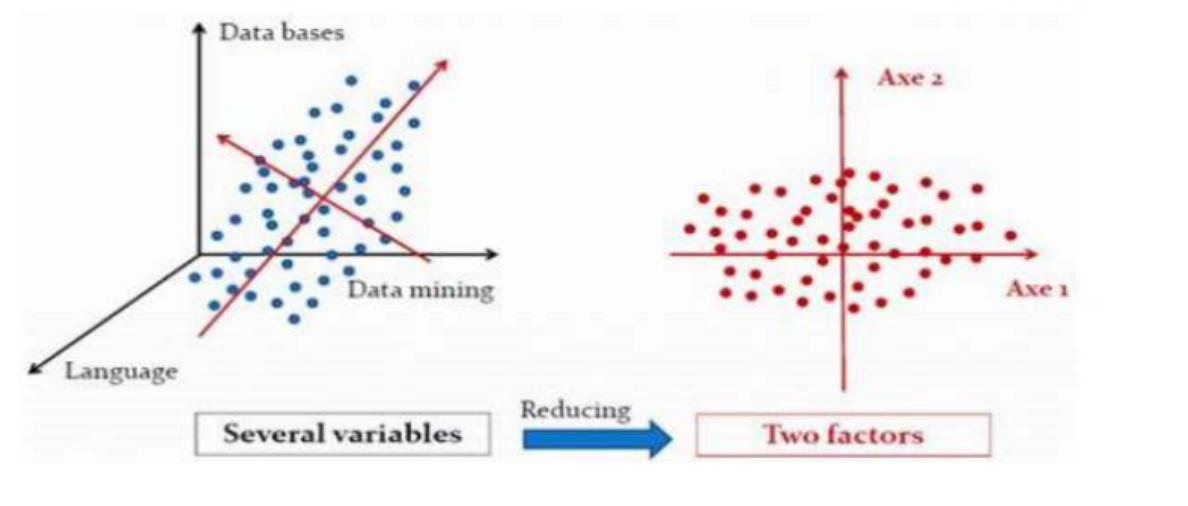
\includegraphics[width = 0.9\textwidth]{2.png}
\end{center}
\begin{itemize}
    \item[b)] Đặc tính:
\end{itemize}

\textul{\textit{Giảm chiều dữ liệu}}: Giảm chiều dữ liệu bằng cách chọn ra những thành phần chính quan trọng nhất giúp giảm thiểu sực phức tap của dữ liệu và làm cho việc xử lý trở nên dễ dàng hơn.

\textul{\textit{Ít ảnh hưởng bởi nhiễu}}: Loại bỏ các biến không quan trọng trong dữ liệu có sự tương quan với nhau, giúp làm sạch và tránh gây nhiễu thông tin.

\textul{\textit{Tăng hiệu suất tính toán}}: Giảm số lượng tính toán bằng cách giảm số chiều của dữ liệu tối ưu hóa thời gian tính toán và tài nguyên máy tính để xử lý dữ liệu.

\textul{\textit{Khả năng trực quan hóa}}: PCA cho phép trực quan hóa dữ liệu trong không gian giảm chiều để hiểu được cấu trúc dữ liệu một cách trực quan.

\textul{\textit{Về mặt ý nghĩa toán học}}: PCA giúp chúng ta xây dựng những biến mới là tổ hợp tuyến tính của những biến ban đầu.
\begin{itemize}
    \item Do PCA giúp tạo 1 hệ trục tọa độ mới nên về mặt ngữ nghĩa toán học, PCA giúp chúng ta xây dựng những biến factor mới là tổ hợp tuyến tính của những biến ban đầu.
    \item Do dữ liệu ban đầu lớn (nhiều biến) thì PCA giúp chúng ta xoay trục tọa độ, xây dựng một hệ tọa độ mới đảm bảo độ biến thiên dữ liệu và dữ lại nhiều thông tin nhất mà không ảnh hưởng đến chất lượng của mô hình dự báo.
    \item Trong không gian mới, chúng ta có thể khám phá thêm những thông tin quý giá mà tại chiều không gian cũ những thông tin này bị che mất (Điển hình là ví dụ về chú lạc đà ở phía trên).
\end{itemize}
$\divideontimes$ Phương pháp phân tích thành phần chính PCA đóng vai trò quan trọng và được sử dụng rộng rãi trong các lĩnh vực kinh tế, sinh học, hóa học và nhiều lĩnh vực khác.

\textul{\textit{Các bước phân tích PCA}}

\textbf{Bước 1.} Tính giá trị trung bình X của X, Chuẩn hóa dữ liệu, tìm tọa độ mới của dữ liệu
\begin{center}
    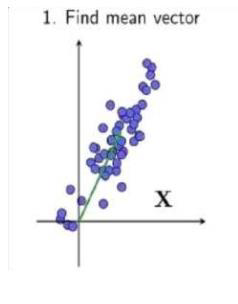
\includegraphics[width = 0.4\textwidth]{3.png}
\end{center}

\textbf{Bước 2.} Tìm vector $\widehat{X} = X - \widehat{X}$. Tính ma trận hiệp phương sai $S = \dfrac{1}{N-1}\widehat{X} \widehat{X}^T$
\begin{center}
    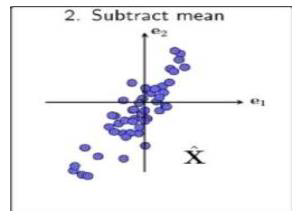
\includegraphics[width = 0.5\textwidth]{4.png}
\end{center}

\textbf{Bước 3.} Tìm trị riêng của S và sắp xếp theo giá trị tăng dần: $\lambda_1 > \lambda_2 > \cdots > \lambda_m$ và tìm các vector riêng đơn vị ứng với các trị riêng.

\textbf{Bước 4.} Chọn K trị riêng ban dầu và K vector trị riêng đơn vị tương ứng. Lập ma trận A có các cột là các vector riêng đã chọn. Ma trận A là phép biến đổi cần tìm.

\begin{center}
    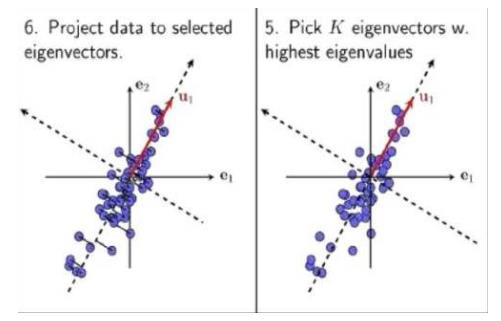
\includegraphics[width = 0.5\textwidth]{5.png}
\end{center}

\textbf{Bước 5.} Tính ảnh $\widehat{A}^T \widehat{X}^T$ của vecto $\widehat{X}$

Dữ liệu X ban đầu được xấp xỉ bởi $X \approx A\widehat{X} + \overline{X}$

Mỗi cột của $A\widehat{X}^T$ chứa tọa độ của các hàng của ma trận $\widehat{X}$ trong cơ sở từ các cột của ma trận P (P là ma trận trực giao).

\textbf{Lưu ý:}
\begin{itemize}
    \item[+] Ma trận S là ma trận đối xứng và các giá trị riêng của S là các số thực không âm.
    \item[+] Ma trận S luôn chéo hóa trực giao được
    \item[+] Trên đường chéo của S là phương sai của các vector $x_1, x_2, \cdots x_N$.
    
    Phần tử $s_{ij}$ là hiệp phương sai của $x_i$ và $x_j$

    Tổng các phần tử trên đường chéo của D là phương sai của bảng dữ liệu.

    Giả sử S=PD$\text{P}^\text{T}$. Trên đường chéo của D là các giá trị riêng của S

    Tổng các giá trị riêng của S bằng tổng các phần tử của S (bằng vết của S).
    \item[+] Ma trận P là ma trận trực giao. Mỗi ma trận trực giao tương ứng với một phép quay.
    
    Các cột của ma trận P tạo nên hệ trực chuẩn. Nếu ta chọn cở sở trực chuẩn là học vector cột của ma trận P, thì ta xây dựng được hệ trục tọa độ mới dựa trên các vector này và có một phép quay từ hệ trục tọa độ ban đầu sang hệ trục tọa độ mới.
    \item[+] Nếu dữ liệu mẫu (Sample data) thì $S = \frac{1}{N-1}\widehat{X}^T \widehat{X}$.
    \item[+] Nếu dữ liệu dân số (Population data) thì $S = \frac{1}{N}\widehat{X}^T \widehat{X}$.
\end{itemize}

\subsubsection{Mục đích của phân tích PCA}
\textul{\textit{Ý tưởng chính}}

Nhận diện khuôn mặt có thể hiểu là một hệ thống dùng để tự động phân tích, loại trừ và xác định, nhận dạng khuôn mặt dựa trên dữ liệu đầu vào là hình ảnh kỹ thuật số hoặc một video. Hiểu ngắn gọn thì hệ thống này sẽ phân tích, đưa ra các thông số, đặc điểm và so sánh những dữ liệu ấy với thông số của một cơ sở dữ liệu đã có sẵn.

Những bức ảnh được đưa vào để xử lý thường có độ phân giải (hoặc kích thước theo 2 chiều x và y) rất lớn nên ta cần “nén” hay nói cách khác là giảm đi độ phân giải (hoặc chiều) của bức ảnh và chỉ giữ lại những thông tin quan trọng nhất, lúc này thuật toán PCA sẽ thực hiện công việc ấy

\textul{\textit{Mục tiêu chính của phương pháp PCA}}

Giảm số chiều của 1 tập vectơ.

Đảm bảo giữ lại được tối đa những thông tin quan trọng nhất của khuôn mặt.
\begin{itemize}
    \item Phân tích và giữ lại k thuộc tính mới của khuôn mặt (Feature Extraction)
    \item Bỏ đi những thuộc tính chung (ban đầu) với những khuôn mặt khác
\end{itemize}
\begin{center}
    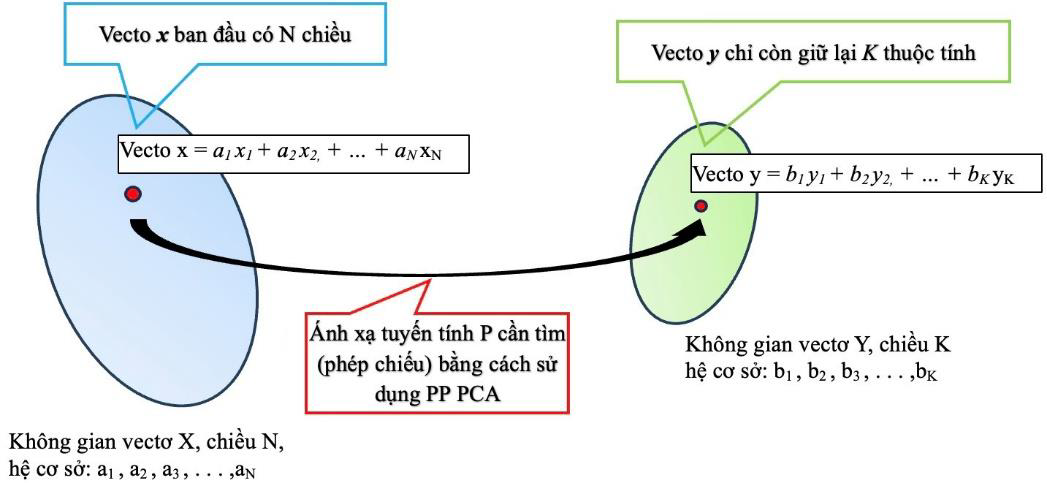
\includegraphics[width = 0.9\textwidth]{6.png}
\end{center}
\subsubsection{Ứng dụng của PCA trong nhận diện khuôn mặt}
VD: Eigen faces

\textul{\textbf{Tiền xử lý}}: Đưa kích cỡ của các hình ảnh về chung kích thước chuẩn hóa (x * y) hoặc (x * x), tạo thành một CSDL input để xử lý

\textul{\textbf{Tách khuôn mặt}}: Tách phần khuôn mặt cần nhận diện trong ảnh, các khuôn mặt này sẽ được sử dụng để tạo thành một bản đồ các vecto.

\textul{\textbf{Chọn lọc đặt trưng khuôn mặt k}}: Tìm các đặc trưng chính của mặt trong ảnh, từ đó tạo nên các vecto đặc trưng cho khuôn mặt, ta sắp xếp các vecto này thành một ma trận để so sánh giữa các đặc điểm giữa khuôn mặt trong ảnh và khuôn mặt có trong CSDL.

\textul{\textbf{So sánh}}: So sánh các vecto đặc trưng trong ma trận, tìm sự tương đồng lớn nhất trong cơ sở dữ liệu và ảnh lưu trữ trong CSDL.
\begin{center}
    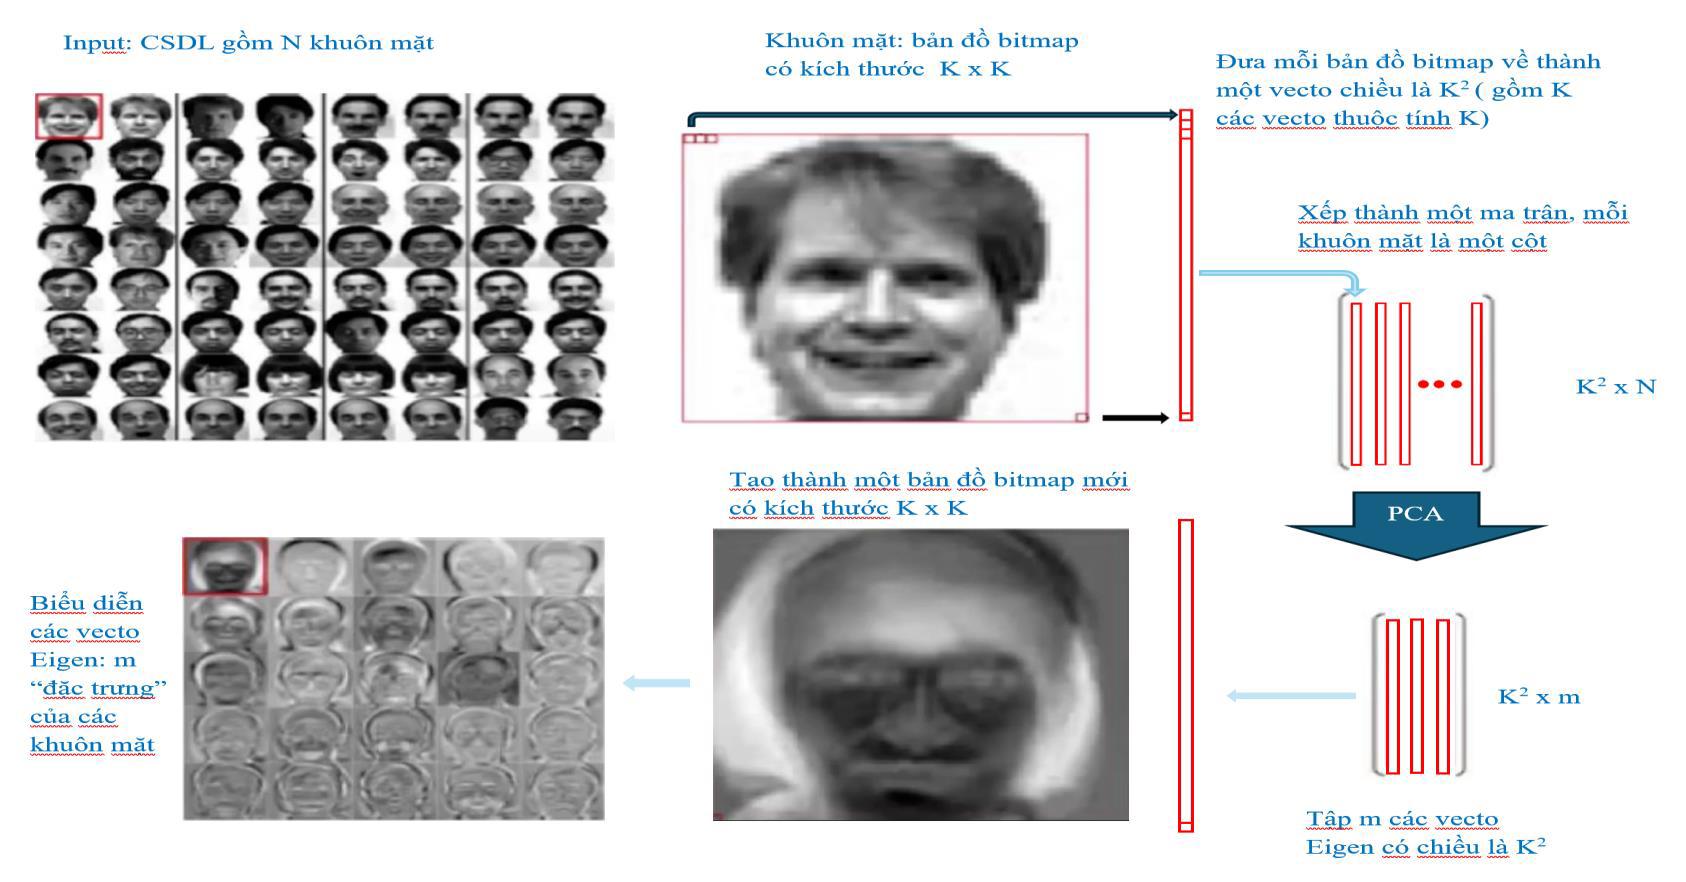
\includegraphics[width = 1\textwidth]{7.png}
\end{center}
\textul{\textit{Ứng dụng thực tế PCA:}}
\begin{itemize}
    \item Nhận dạng khuôn mặt trên chứng minh thư nhân dân
    \item Hệ thống theo dõi an ninh, quan sát , bảo vệ trong các toà nhà, cơ quan
    \item Kiểm tra trạng thái tỉnh táo của người lái xe và cảnh bảo kịp thời
    \item Giao tiếp giữa con người và máy móc
    \item Phân loại, nhận diện người trong các hình ảnh trong điện thoại di động
    \item Robot hỗ trợ bệnh nhân
    \item Giải pháp bảo mật không dùng mã pin cho các giao dịch rút tiền tại các ATM
    \item Tìm kiếm, hỗ trợ, tổ chức, tạo cơ sở dữ liệu người trong tổ chức trong các hệ cơ sở dữ liệu quốc gia, internet
    \item Theo dõi khuôn mặt trong quay video
    \item Hỗ trợ tập trung trong các máy ảnh kĩ thuật số
    \item Hệ thống hỗ trợ tìm kiếm người thất lạc, $\cdots$

\end{itemize}

\subsubsection{Ưu điểm của PCA}
PCA giúp giảm thiểu số lượng biến cần thiết trong phân tích, từ đó giảm thời gian tính toán và tăng hiệu suất cho các thuật toán học máy.

Kỹ thuật này có thể làm nổi bật các cấu trúc và mẫu trong dữ liệu, giúp các nhà nghiên cứu và nhà phát triển dễ dàng hơn trong việc phân tích và diễn giải.

PCA có khả năng loại bỏ các biến không quan trọng, từ đó làm cho mô hình trở nên đơn giản và dễ giải thích hơn.

PCA có thể giúp xác định các mối quan hệ ẩn giữa các biến trong dữ liệu, điều này có thể mang lại thông tin giá trị cho các ứng dụng khác nhau.
\subsubsection{Nhược điểm của PCA}
PCA yêu cầu dữ liệu đầu vào phải được chuẩn hóa, nếu không sẽ dẫn đến những kết quả sai lệch trong việc xác định các thành phần chính.

PCA có thể không duy trì được các đặc trưng địa phương của dữ liệu, dẫn đến việc mất mát thông tin quan trọng.

Kết quả của PCA phụ thuộc vào các giá trị riêng và vectơ riêng, khiến cho việc giải thích các thành phần chính trở nên khó khăn trong một số trường hợp.

PCA thường không hiệu quả trong việc xử lý dữ liệu phi tuyến, vì nó chỉ tìm ra các thành phần chính theo một cách tuyến tính. 

Khi dữ liệu có nhiều biến, PCA có nguy cơ gây ra hiện tượng ``overfitting'', đặc biệt khi số lượng mẫu không đủ lớn so với số lượng biến.
\section{THUẬT TOÁN VÀ CODE MATLAB TRONG PHÂN TÍCH PCA ĐỂ NHẬN DIỆN KHUÔN MẶT}
\subsection{Một số lệnh cơ bản được sử dụng}
zeros(): Tạo ma trận với các phần tử bằng 0.

isFile(): Kiểm tra tệp có tồn tại hay không.

imread(): Đọc tệp ảnh.

imresize(): Thay đổi kích thước ảnh.

rgb2gray(): Chuyển đổi sang ảnh grayscale

subplot(): Tạo một subplot để hiển thị nhiều hình ảnh trên cùng một figure.

imshow(): Hiển thị hình ảnh.

title(): Đặt tiêu đề cho subplot.

error(): Hiển thị thông báo lỗi và dừng thực thi chương trình.

mean(): Tính giá trị trung bình.

sort(): Sắp xếp các phần tử.

min(): Tìm giá trị nhỏ nhất.

fprintf(): In ra màn hình.
\subsection{Đoạn code sử dụng trong matlab}
\begin{center}
    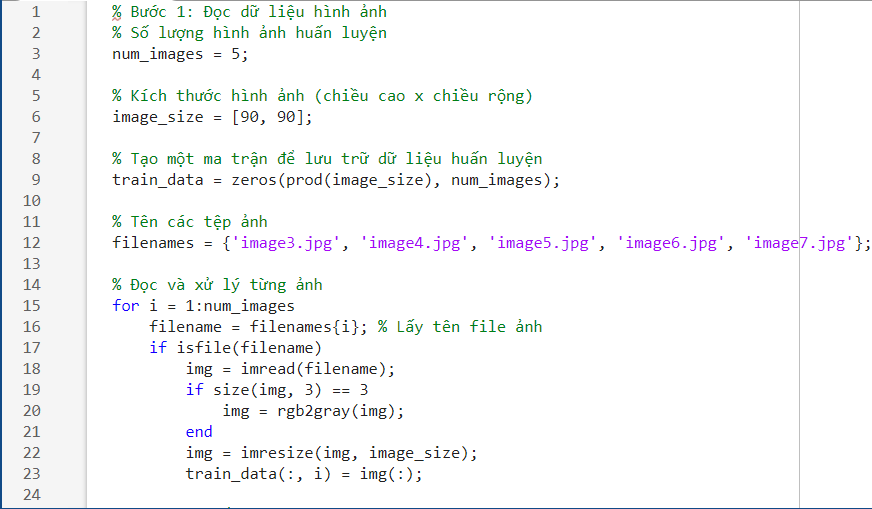
\includegraphics[width = 1\textwidth]{8.png}
\end{center}
\begin{center}
    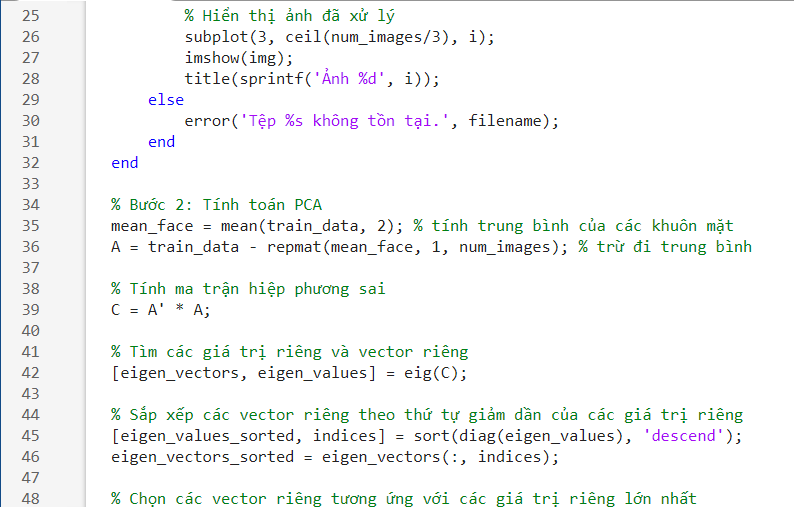
\includegraphics[width = 1\textwidth]{9.png}
\end{center}
\begin{center}
    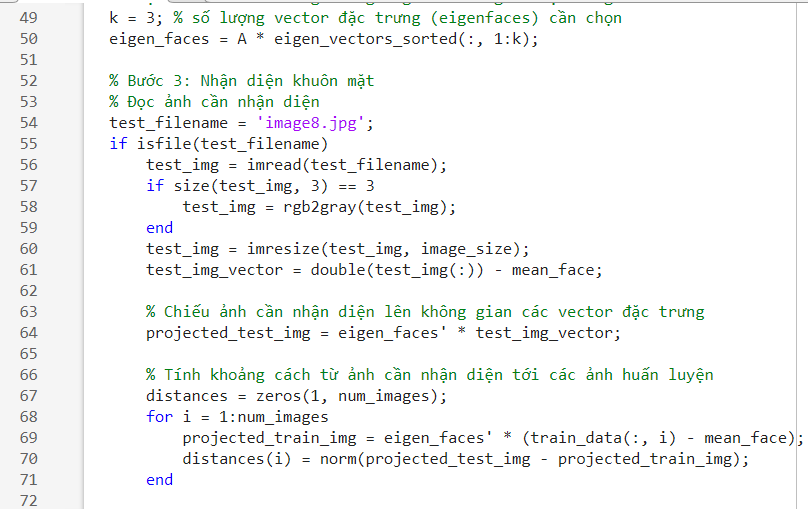
\includegraphics[width = 1\textwidth]{10.png}
\end{center}
\begin{center}
    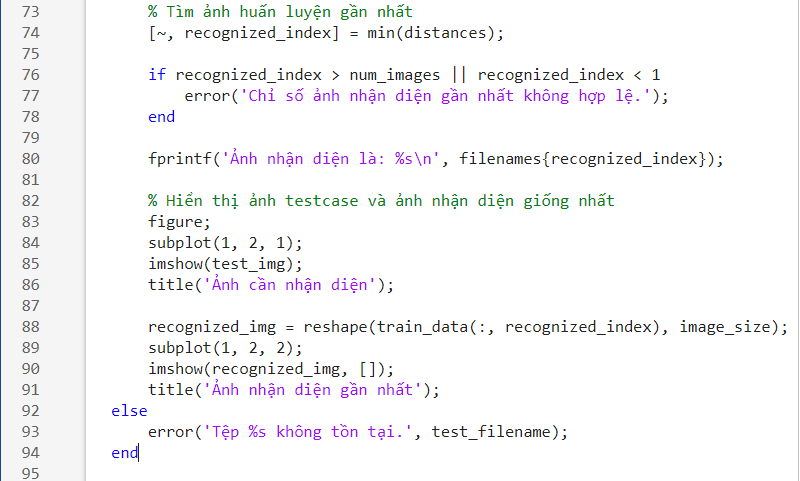
\includegraphics[width = 1\textwidth]{11.png}
\end{center}
\subsection{Ví dụ minh họa}
Chuẩn bị 6 hình ảnh của 3 người khác nhau, đưa vào chương trinh 5 hình ảnh để huấn luyện. Sử dụng hình ảnh còn lại để kiểm tra chương trình. Chương trình sẽ in ra hình ảnh nhận diện gần giống nhất trong 5 hình ảnh huấn luyện. Kết quả:
\begin{center}
    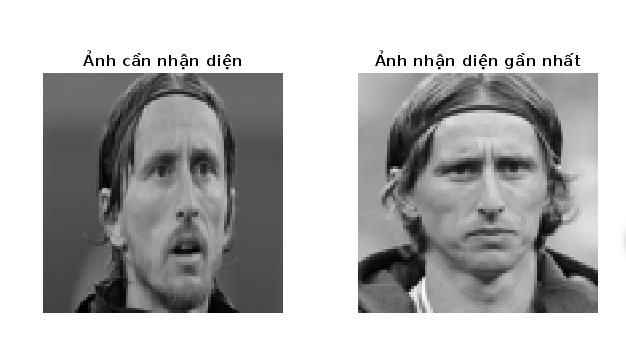
\includegraphics[width = 1\textwidth]{12.png}
\end{center}
\section{KẾT LUẬN}
Trong quá trình làm bài tập lớn về phân tích PCA để nhận diện khuôn mặt, nhóm 03 đã làm rõ và nêu đầy đủ thông tin về các đặc trưng của vector ngẫu nhiên như kỳ vọng, phương sai, độ lệch chuẩn … một cách ngắn gọn và có ví dụ minh họa giúp người đọc dễ hiểu. Tiếp đó, nhóm đã thành công giới thiệu một cách mạch lạc và đầy đủ về phân tích  PCA gồm cách nội dung như: giới thiệu PCA, nêu lên được mục đích sử dụng PCA trong nhận diện khuôn mặt, và chỉ ra được ưu và nhược điểm của việc sử dụng PCA.

Nhưng nhóm cũng còn gặp 1 số khó khăn nhất định trong thời gian làm bài tập lớn,  nhóm không có nhiều ví dụ cho 1 số nội dung lý thuyết khiến người đọc khó khăn trong việc hiểu rõ nội dung nhóm muốn truyền tải. Về phần code matlab phân tích PCA nhận diện khuôn mặt, nhóm chưa có nhiều kinh nghiệm với matlab nên gặp khá nhiều khó khăn trong việc tìm hiểu cũng như áp dụng trong bài tập lớn.
\section{TÀI LIỆU THAM KHẢO}
1. Sách Đại Số Tuyến Tính của tác giả Đặng Văn Vinh (nhà xuất bản ĐHQG TP. Hồ Chí Minh) xuất bản năm 2019.

2. I.T. Jolliffe, Principal Component Analysis. Springer, 2010. (\href{chrome-extension://efaidnbmnnnibpcajpcglclefindmkaj/http://cda.psych.uiuc.edu/statistical_learning_course/Jolliffe%20I.%20Principal%20Component%20Analysis%20(2ed.,%20Springer,%202002)(518s)_MVsa_.pdf}{\textcolor{Danube}{\textul{https://shorturl.at/TltCO}}})

3. Yoshio Takane, Constrained Principal Component Analysis and Related Techniques, Taylor \& Francis Group, LLC. (\href{chrome-extension://efaidnbmnnnibpcajpcglclefindmkaj/https://api.pageplace.de/preview/DT0400.9781466556683_A24034672/preview-9781466556683_A24034672.pdf}{\textcolor{Danube}{\textul{https://shorturl.at/mjFAl}}})
\end{document}